



\begin{frame}{Firmware}
	``Unter Firmware versteht man Software, die in elektronische Geräte eingebettet ist.'' \cite{wikiFirmware}
	
	\begin{itemize}
		\item Geamtes Software-Image von Embedded System
		\item Software fuer subsyteme
		\begin{itemize}
			\item Power Management
			\item WLAN Karte
			\item BIOS
			\item Touch-Screen
		\end{itemize}
	\end{itemize}
	
	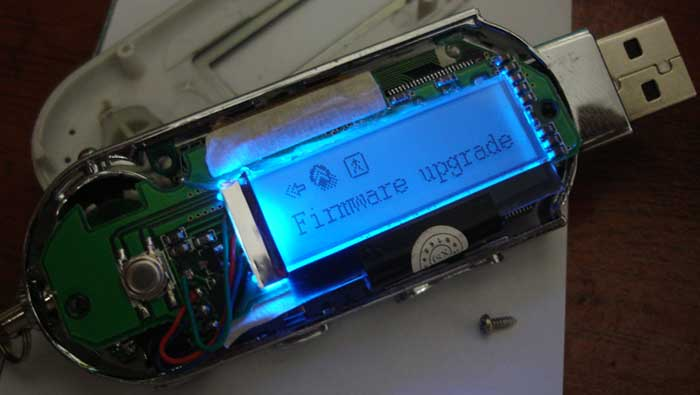
\includegraphics[height=2cm]{res/Firmware_upgrade.jpg} \cite{firmwareUpgrade}
\end{frame}

\begin{frame}{PID 1}
	Nachdem Linux alles initializiert hat wird Kontrolle an Userspace uebergeben.
	Ueblicherweise ist dies systemd.
	\begin{itemize}
		\item systemd
		\begin{itemize}
			\item einfach da bekannt
			\item wenn mehrere Dienste noetig
			\item gewisse groesse
		\end{itemize}
		\item script
		\begin{itemize}
			\item wenn nur wenige Dienste
		\end{itemize}
		\item applikation
		\begin{itemize}
			\item Applikation muss alles machen
			\item nur fuer monolithische Applikationen
		\end{itemize}
	\end{itemize}
\end{frame}

\begin{frame}{Yocto}
	Aufgaben um Embedded system zu erstellen
	\begin{itemize}
		\item Cross Compiler bauen
		\item sysfs bauen (Kernel und benoetigte Tools fuer system)
		\item Cross Compiler und sysfs fuer Developer bereitstellen (sdk)
	\end{itemize}
	Aufgaben um Embedded system zu deployen
	\begin{itemize}
		\item Applikation cross-compilen
		\item sysfs cross-compilen
		\item Kernel cross-compilen
		\item applikationen packetieren
		\item image zusammenstellen
	\end{itemize}
	daher Yocto (Yocto Workflow zeigen, resp. bild aus fsfe präsentation)
\end{frame}

\begin{frame}{Kernel / Linux}
	\begin{itemize}
		\item Verteilen von Resourcen
		\item Initialisieren und Abstrahieren der Hardware
	\end{itemize}
\end{frame}

